\documentclass[12pt]{article}
\usepackage[utf8]{inputenc}
\usepackage[utf8]{vietnam}
\usepackage{amsmath, amssymb, amsfonts}
\usepackage{tikz}
\usetikzlibrary{arrows.meta, calc, angles, quotes}
\usepackage{geometry}
\geometry{a4paper, margin=0.8in}
\usepackage{xcolor}
\usepackage{pifont}
\usepackage[most]{tcolorbox}

% Colors
\definecolor{myblue}{RGB}{0, 102, 204}
\definecolor{myred}{RGB}{204, 0, 0}
\definecolor{highlightyellow}{RGB}{255, 235, 59}

% Custom components
\newcommand{\bluecheck}{%
  \tikz[baseline=-0.5ex]\node[circle,fill=myblue,inner sep=0.5pt,minimum size=10pt]{\textcolor{white}{\fontsize{5}{5}\selectfont\checkmark}};%
}
\newcommand{\handwrite}{\textcolor{myblue}{\ding{46}}}

\newtcolorbox{notebox}[1][]{
  colback=myred!5!white,
  colframe=myred,
  arc=4pt,
  boxrule=0.5pt,
  leftrule=3pt,
  #1
}

\begin{document}

% Header
\begin{center}
    \textcolor{myred}{\small thuvienhoclieu.com} \\
    \vspace{0.2cm}
    \colorbox{highlightyellow}{\textbf{\color{myred}{\large\quad CHỦ ĐỀ 8. HÌNH HỌC KHÔNG GIAN\quad}}}
\end{center}

\vspace{0.3cm}

\noindent\textbf{\color{myblue}{\large A. KIẾN THỨC CẦN NHỚ}}\\
\noindent\textbf{\color{myblue}{\large I. QUAN HỆ SONG SONG TRONG KHÔNG GIAN}}\\

\noindent\textbf{\color{myblue}{1. Giao tuyến của 2 mp:}} Đường thẳng $d$ chung của hai mặt phẳng $(P)$ và $(Q)$ được gọi là giao tuyến của $(P)$ và $(Q)$, kí hiệu $d = (P) \cap (Q)$.\\

\noindent\textbf{\color{myblue}{2. Thiết diện:}} Thiết diện của mặt phẳng $\underline{(\alpha)}$ với hình chóp $\underline{(H)}$ là phần chung giữa mặt phẳng $\underline{(\alpha)}$ và hình chóp $\underline{(H)}$.\\

\noindent\textbf{\color{myblue}{3. Vị trí tương đối của hai đường thẳng trong không gian}}\\
\textit{TH1: $a$ và $b$ đồng phẳng}
\begin{itemize}
    \item[\bluecheck] $a$ cắt $b \Leftrightarrow a \cap b = \{M\}$.
    \item[\bluecheck] $a \parallel b \Leftrightarrow a \cap b = \varnothing$.
    \item[\bluecheck] $a \equiv b \Leftrightarrow a \cap b = a$.
\end{itemize}
\textit{TH2: không có mp nào chứa $a$ và $b$, ta nói \textbf{\color{myblue}{$a$ và $b$ chéo nhau}}.}

\vspace{0.4cm}

% 4 Diagrams for relative positions of two lines
\begin{center}
\begin{tabular}{cccc}
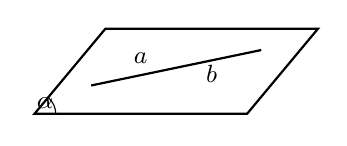
\begin{tikzpicture}[scale=0.9, >=stealth]
  \draw[thick] (0,0) -- (3,0) -- (4,1.2) -- (1,1.2) -- cycle;
  \draw (0.3,0) arc (0:50:0.3);
  \node at (0.15,0.15) {\small $\alpha$};
  \draw[thick] (0.8,0.4) -- (3.2,0.9);
  \node[above] at (1.5,0.57) {\small $a$};
  \node[below] at (2.5,0.82) {\small $b$};
\end{tikzpicture}
&
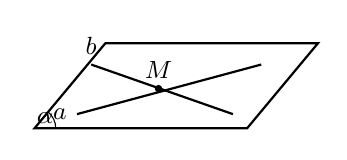
\begin{tikzpicture}[scale=0.9, >=stealth]
  \draw[thick] (0,0) -- (3,0) -- (4,1.2) -- (1,1.2) -- cycle;
  \draw (0.3,0) arc (0:50:0.3);
  \node at (0.15,0.15) {\small $\alpha$};
  \draw[thick] (0.6,0.2) node[left] {\small $a$} -- (3.2,0.9);
  \draw[thick] (0.8,0.9) node[above] {\small $b$} -- (2.8,0.2);
  \coordinate (M) at (1.75,0.56);
  \fill (M) circle (1.5pt);
  \node[above] at (1.75,0.56) {\small $M$};
\end{tikzpicture}
&
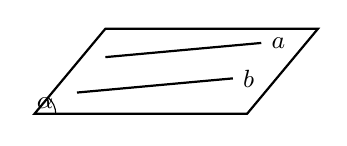
\begin{tikzpicture}[scale=0.9, >=stealth]
  \draw[thick] (0,0) -- (3,0) -- (4,1.2) -- (1,1.2) -- cycle;
  \draw (0.3,0) arc (0:50:0.3);
  \node at (0.15,0.15) {\small $\alpha$};
  \draw[thick] (1.0,0.8) -- (3.2,1.0) node[right] {\small $a$};
  \draw[thick] (0.6,0.3) -- (2.8,0.5) node[right] {\small $b$};
\end{tikzpicture}
&
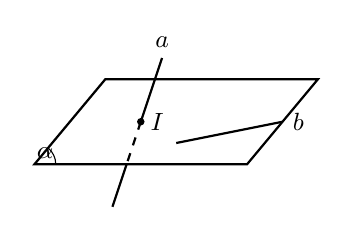
\begin{tikzpicture}[scale=0.9, >=stealth]
  \draw[thick] (0,0) -- (3,0) -- (4,1.2) -- (1,1.2) -- cycle;
  \draw (0.3,0) arc (0:50:0.3);
  \node at (0.15,0.15) {\small $\alpha$};
  \draw[thick] (2.0,0.3) -- (3.5,0.6) node[right] {\small $b$};
  \coordinate (I) at (1.5,0.6);
  \draw[thick] (1.8,1.5) node[above] {\small $a$} -- (I);
  \draw[dashed, thick] (I) -- (1.3,0);
  \draw[thick] (1.3,0) -- (1.1,-0.6);
  \fill (I) circle (1.5pt) node[right] {\small $I$};
\end{tikzpicture}
\\
$a \equiv b$ & $a \cap b = \{M\}$ & $a \parallel b$ & $a, b$ chéo nhau \\
a) & b) & c) & d)
\end{tabular}
\end{center}

\vspace{0.4cm}

\noindent\textbf{\color{myblue}{a/ Hai đường thẳng song song:}} nếu chúng cùng nằm trên một mặt phẳng và không có điểm chung.

\begin{notebox}
\noindent\textbf{\color{myred}{\textit{*Chú ý:}}}\\
\indent 1. Hai đường thẳng gọi là \textit{chéo nhau} nếu chúng không đồng phẳng.\\
\indent 2. Cho hai đường thẳng song song $a$ và $b$. Có duy nhất một mặt phẳng chứa hai đường thẳng đó, kí hiệu $\text{mp}(a, b)$.
\end{notebox}

\vspace{0.2cm}

\noindent\textbf{\color{myblue}{b/ Tính chất cơ bản về hai đường thẳng song song.}}\\
\textbf{+} Nếu ba mp phân biệt đôi một cắt nhau theo ba giao tuyến phân biệt thì ba giao tuyến ấy hoặc đồng quy hoặc đôi một song song với nhau.

\vspace{0.4cm}

% 2 Diagrams for 3 planes intersection (Point intersection & Parallel lines)
\begin{center}
\begin{tabular}{cc}
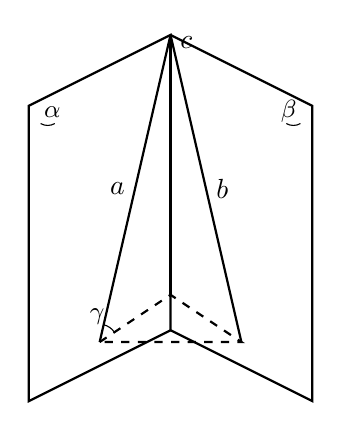
\begin{tikzpicture}[scale=1.5, >=stealth]
  \coordinate (V) at (0,2);
  \coordinate (O) at (0,-0.5);
  \coordinate (TL) at (-1.2, 1.4);
  \coordinate (BL) at (-1.2, -1.1);
  \coordinate (TR) at (1.2, 1.4);
  \coordinate (BR) at (1.2, -1.1);

  \draw[thick] (TL) -- (V) -- (O) -- (BL) -- cycle;
  \draw[thick] (V) -- (TR) -- (BR) -- (O);

  \draw (-1.1, 1.25) arc (240:300:0.12);
  \node at (-1.0, 1.35) {\small $\alpha$};
  
  \draw (1.1, 1.25) arc (300:240:0.12);
  \node at (1.0, 1.35) {\small $\beta$};

  \coordinate (A0) at (-0.6, -0.6);
  \coordinate (B0) at (0.6, -0.6);
  \coordinate (C0) at (0, -0.2);

  \draw[dashed, thick] (A0) -- (C0) -- (B0) -- cycle;

  \draw[thick] (A0) -- (V) node[midway, left] {$a$};
  \draw[thick] (B0) -- (V) node[midway, right] {$b$};
  \draw[thick] (C0) -- (V);
  \node[above right] at (0, 1.8) {$c$};

  \draw (-0.6, -0.6) + (34:0.15) arc (34:77:0.15);
  \node at (-0.62, -0.38) {\small $\gamma$};
\end{tikzpicture}
&
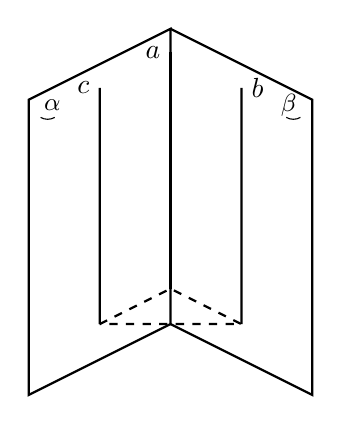
\begin{tikzpicture}[scale=1.5, >=stealth]
  \coordinate (V) at (0,2);
  \coordinate (O) at (0,-0.5);
  \coordinate (TL) at (-1.2, 1.4);
  \coordinate (BL) at (-1.2, -1.1);
  \coordinate (TR) at (1.2, 1.4);
  \coordinate (BR) at (1.2, -1.1);

  \draw[thick] (TL) -- (V) -- (O) -- (BL) -- cycle;
  \draw[thick] (V) -- (TR) -- (BR) -- (O);

  \draw (-1.1, 1.25) arc (240:300:0.12);
  \node at (-1.0, 1.35) {\small $\alpha$};
  
  \draw (1.1, 1.25) arc (300:240:0.12);
  \node at (1.0, 1.35) {\small $\beta$};

  \coordinate (C0) at (-0.6, -0.5);
  \coordinate (B0) at (0.6, -0.5);
  \coordinate (A0) at (0, -0.2);

  \draw[dashed, thick] (C0) -- (A0) -- (B0) -- cycle;

  \draw[thick] (C0) -- (-0.6, 1.5) node[left] {$c$};
  \draw[thick] (B0) -- (0.6, 1.5) node[right] {$b$};
  \draw[thick] (A0) -- (0, 1.8) node[left] {$a$};
\end{tikzpicture}
\end{tabular}
\end{center}

\vspace{0.4cm}

\noindent\textbf{+} Nếu hai mp phân biệt lần lượt chứa hai đt song song thì giao tuyến của chúng (nếu có) cũng song song với hai đt đó hoặc trùng với một trong hai đt đó.

\vspace{0.4cm}

% 3 Diagrams for parallel lines in intersecting planes
\begin{center}
\begin{tabular}{ccc}
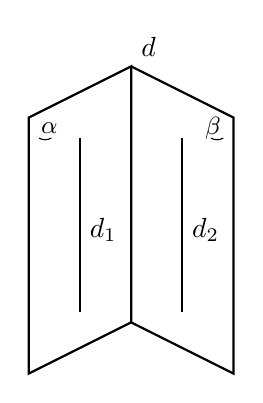
\begin{tikzpicture}[scale=1.3, >=stealth]
  \coordinate (V) at (0,2);
  \coordinate (O) at (0,-0.5);
  \coordinate (TL) at (-1.0, 1.5);
  \coordinate (BL) at (-1.0, -1.0);
  \coordinate (TR) at (1.0, 1.5);
  \coordinate (BR) at (1.0, -1.0);

  \draw[thick] (TL) -- (V) -- (O) -- (BL) -- cycle;
  \draw[thick] (V) -- (TR) -- (BR) -- (O);

  \draw (-0.9, 1.3) arc (240:300:0.12);
  \node at (-0.8, 1.4) {\small $\alpha$};
  \draw (0.9, 1.3) arc (300:240:0.12);
  \node at (0.8, 1.4) {\small $\beta$};

  \draw[thick] (0, -0.5) -- (0, 2) node[above right] {$d$};
  \draw[thick] (-0.5, -0.4) -- (-0.5, 1.3);
  \node[right] at (-0.5, 0.4) {$d_1$};
  \draw[thick] (0.5, -0.4) -- (0.5, 1.3);
  \node[right] at (0.5, 0.4) {$d_2$};
\end{tikzpicture}
&
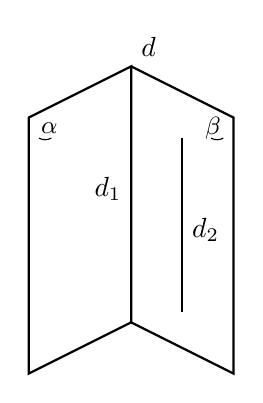
\begin{tikzpicture}[scale=1.3, >=stealth]
  \coordinate (V) at (0,2);
  \coordinate (O) at (0,-0.5);
  \coordinate (TL) at (-1.0, 1.5);
  \coordinate (BL) at (-1.0, -1.0);
  \coordinate (TR) at (1.0, 1.5);
  \coordinate (BR) at (1.0, -1.0);

  \draw[thick] (TL) -- (V) -- (O) -- (BL) -- cycle;
  \draw[thick] (V) -- (TR) -- (BR) -- (O);

  \draw (-0.9, 1.3) arc (240:300:0.12);
  \node at (-0.8, 1.4) {\small $\alpha$};
  \draw (0.9, 1.3) arc (300:240:0.12);
  \node at (0.8, 1.4) {\small $\beta$};

  \draw[thick] (0, -0.5) -- (0, 2) node[above right] {$d$};
  \node[left] at (0, 0.8) {$d_1$};
  \draw[thick] (0.5, -0.4) -- (0.5, 1.3);
  \node[right] at (0.5, 0.4) {$d_2$};
\end{tikzpicture}
&
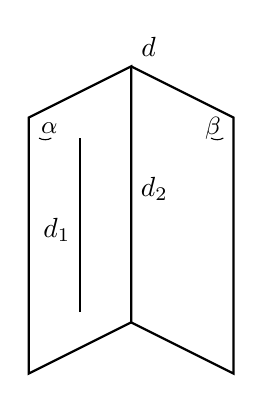
\begin{tikzpicture}[scale=1.3, >=stealth]
  \coordinate (V) at (0,2);
  \coordinate (O) at (0,-0.5);
  \coordinate (TL) at (-1.0, 1.5);
  \coordinate (BL) at (-1.0, -1.0);
  \coordinate (TR) at (1.0, 1.5);
  \coordinate (BR) at (1.0, -1.0);

  \draw[thick] (TL) -- (V) -- (O) -- (BL) -- cycle;
  \draw[thick] (V) -- (TR) -- (BR) -- (O);

  \draw (-0.9, 1.3) arc (240:300:0.12);
  \node at (-0.8, 1.4) {\small $\alpha$};
  \draw (0.9, 1.3) arc (300:240:0.12);
  \node at (0.8, 1.4) {\small $\beta$};

  \draw[thick] (0, -0.5) -- (0, 2) node[above right] {$d$};
  \node[right] at (0, 0.8) {$d_2$};
  \draw[thick] (-0.5, -0.4) -- (-0.5, 1.3);
  \node[left] at (-0.5, 0.4) {$d_1$};
\end{tikzpicture}
\\
a) & b) & c)
\end{tabular}
\end{center}

\vspace{0.4cm}

\noindent\handwrite\ \textbf{\color{myblue}{+ Hai đường thẳng phân biệt cùng song song với đường thẳng thứ ba thì song song với nhau.}}
\[
\begin{cases}
a \neq b \\
a \parallel c \\
b \parallel c
\end{cases}
\Rightarrow a \parallel b
\]

\newpage

% Page 2 content starts here
\noindent\textbf{\color{myblue}{\large 4. Vị trí tương đối của đường thẳng và mặt phẳng}}\\
Cho đường thẳng $a$ và mặt phẳng $(P)$. Khi đó có thể xảy ra một trong ba trường hợp sau:

\noindent\textbf{+ TH 1:} $a$ và $(P)$ có từ hai điểm chung phân biệt trở lên (Hình 2a), suy ra mọi điểm thuộc $a$ đều thuộc $(P)$, ta nói $a$ nằm trong $(P)$, kí hiệu $a \subset (P)$.

\noindent\textbf{+ TH 2:} $a$ và $(P)$ có một điểm chung duy nhất $A$ (Hình 2b), ta nói $a$ cắt $(P)$ tại $A$, kí hiệu $a \cap (P) = \{A\}$.

\noindent\textbf{+ TH 3:} $a$ và $(P)$ không có điểm chung nào (Hình 2c), ta nói $a$ song song với $(P)$, kí hiệu $a \parallel (P)$.

\vspace{0.4cm}

% 3 Diagrams for line & plane relative positions
\begin{center}
\begin{tabular}{ccc}
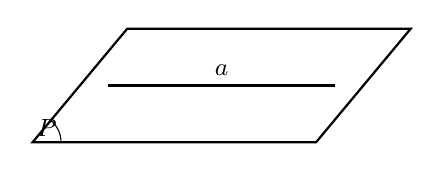
\begin{tikzpicture}[scale=1.2, >=stealth]
  \draw[thick] (0,0) -- (3,0) -- (4,1.2) -- (1,1.2) -- cycle;
  \draw (0.3,0) arc (0:50:0.3);
  \node at (0.15,0.15) {\small $P$};
  \draw[thick] (0.8, 0.6) -- (3.2, 0.6);
  \node[above] at (2.0, 0.6) {\small $a$};
\end{tikzpicture}
&
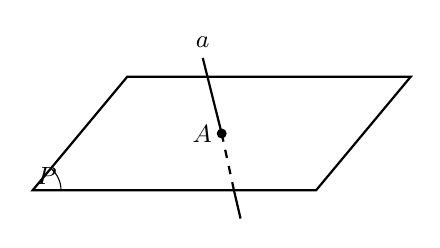
\begin{tikzpicture}[scale=1.2, >=stealth]
  \draw[thick] (0,0) -- (3,0) -- (4,1.2) -- (1,1.2) -- cycle;
  \draw (0.3,0) arc (0:50:0.3);
  \node at (0.15,0.15) {\small $P$};
  
  \coordinate (A) at (2.0, 0.6);
  \draw[thick] (1.8, 1.4) node[above] {\small $a$} -- (A);
  \draw[dashed, thick] (A) -- (2.13, 0);
  \draw[thick] (2.13, 0) -- (2.2, -0.3);
  
  \fill (A) circle (1.5pt) node[left] {\small $A$};
\end{tikzpicture}
&
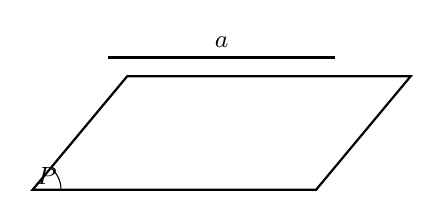
\begin{tikzpicture}[scale=1.2, >=stealth]
  \draw[thick] (0,0) -- (3,0) -- (4,1.2) -- (1,1.2) -- cycle;
  \draw (0.3,0) arc (0:50:0.3);
  \node at (0.15,0.15) {\small $P$};
  \draw[thick] (0.8, 1.4) -- (3.2, 1.4);
  \node[above] at (2.0, 1.4) {\small $a$};
\end{tikzpicture}
\\
Hình 2a & Hình 2b & Hình 2c
\end{tabular}
\end{center}

\vspace{0.4cm}

\noindent\textbf{\color{myblue}{a/ Đường thẳng song song mặt phẳng:}} $a \parallel (P)$ nếu chúng không có điểm chung.

\noindent\textbf{\color{myblue}{b/ Điều kiện để một đường thẳng song song với 1 mặt phẳng}}\\
\textbf{+} Nếu đường thẳng $d$ không nằm trong mặt phẳng $(\alpha)$ và $d$ song song với đường thẳng $d'$ nằm trong $(\alpha)$ thì $d$ song song với $(\alpha)$.

\vspace{0.3cm}

\begin{center}
\begin{minipage}{0.45\textwidth}
\[
\begin{cases}
d \not\subset (\alpha) \\
d \parallel d' \\
d' \subset (\alpha)
\end{cases}
\Rightarrow d \parallel (\alpha)
\]
\end{minipage}
\hfill
\begin{minipage}{0.45\textwidth}
\begin{center}
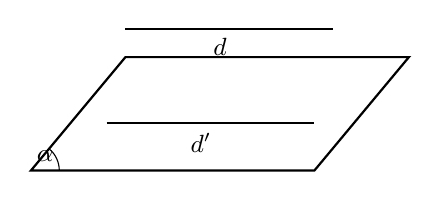
\begin{tikzpicture}[scale=1.2, >=stealth]
  \draw[thick] (0,0) -- (3,0) -- (4,1.2) -- (1,1.2) -- cycle;
  \draw (0.3,0) arc (0:50:0.3);
  \node at (0.15,0.15) {\small $\alpha$};
  \draw[thick] (0.8, 0.5) -- (3.0, 0.5);
  \node[below] at (1.8, 0.5) {\small $d'$};
  \draw[thick] (1.0, 1.5) -- (3.2, 1.5);
  \node[below] at (2.0, 1.5) {\small $d$};
\end{tikzpicture}
\end{center}
\end{minipage}
\end{center}

\vspace{0.4cm}

\noindent\textbf{\color{myblue}{c/ Tính chất cơ bản của đường thẳng và mặt phẳng song song}}\\
\textbf{+} Cho đường thẳng $d$ song song với mặt phẳng $(\alpha)$. Nếu mặt phẳng $(\beta)$ đi qua $d$ và cắt $(\alpha)$ theo giao tuyến $d'$ thì $d' \parallel d$.

\vspace{0.3cm}

\begin{center}
\begin{minipage}{0.45\textwidth}
\[
\begin{cases}
d \parallel (\alpha) \\
d \subset (\beta) \\
(\alpha) \cap (\beta) = d'
\end{cases}
\Rightarrow d' \parallel d
\]
\end{minipage}
\hfill
\begin{minipage}{0.45\textwidth}
\begin{center}
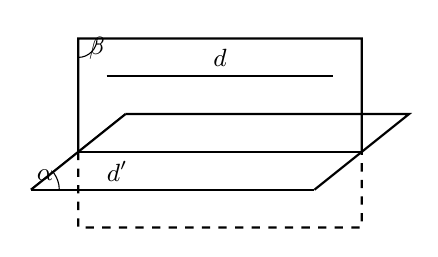
\begin{tikzpicture}[scale=1.2, >=stealth]
  % Coordinates for Plane alpha (horizontal)
  \coordinate (A_TL) at (1.0, 0.4);
  \coordinate (A_TR) at (4.0, 0.4);
  \coordinate (A_BR) at (3.0, -0.4);
  \coordinate (A_BL) at (0, -0.4);
  
  % Draw plane alpha (back and sides)
  \draw[thick] (A_TL) -- (A_TR) -- (A_BR);
  \draw[thick] (A_BL) -- (A_TL);
  
  % Coordinates for Plane beta (vertical)
  \coordinate (B_BL) at (0.5, -0.8);
  \coordinate (B_BR) at (3.5, -0.8);
  \coordinate (B_TL) at (0.5, 1.2);
  \coordinate (B_TR) at (3.5, 1.2);
  
  % Draw upper part of beta
  \draw[thick] (0.5, 0) -- (B_TL) -- (B_TR) -- (3.5, 0);
  % Draw lower part of beta
  \draw[dashed, thick] (0.5, 0) -- (B_BL) -- (B_BR) -- (3.5, 0);
  
  % Draw front edge of alpha
  \draw[thick] (A_BR) -- (A_BL);
  
  % Labels
  \draw (0.3, -0.4) arc (0:38:0.3);
  \node at (0.15, -0.25) {\small $\alpha$};
  
  \draw (0.5, 1.0) arc (-90:0:0.2);
  \node at (0.7, 1.1) {\small $\beta$};
  
  \draw[thick] (0.8, 0.8) -- (3.2, 0.8);
  \node[above] at (2.0, 0.8) {\small $d$};
  
  \draw[thick] (0.5, 0) -- (3.5, 0);
  \node[below right] at (0.7, 0) {\small $d'$};
\end{tikzpicture}
\end{center}
\end{minipage}
\end{center}

\vspace{0.4cm}

\noindent\textbf{+} Nếu hai mặt phẳng phân biệt cùng song song với một đường thẳng thì giao tuyến của chúng (nếu có) cũng song song với đường thẳng đó.

\vspace{0.4cm}

\begin{center}
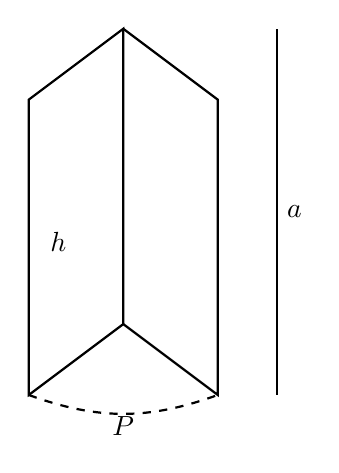
\begin{tikzpicture}[scale=1.5, >=stealth]
  \coordinate (V) at (0,2);
  \coordinate (O) at (0,-0.5);
  \coordinate (TL) at (-0.8, 1.4);
  \coordinate (BL) at (-0.8, -1.1);
  \coordinate (TR) at (0.8, 1.4);
  \coordinate (BR) at (0.8, -1.1);

  \draw[thick] (TL) -- (V) -- (O) -- (BL) -- cycle;
  \draw[thick] (V) -- (TR) -- (BR) -- (O);

  \draw[dashed, thick] (O) -- (V);
  \draw[dashed, thick] (BL) to[out=-20, in=200] (BR);

  \draw[thick] (1.3, -1.1) -- (1.3, 2.0) node[midway, right] {$a$};

  \node[left] at (-0.4, 0.2) {$h$};
  \node[below] at (0, -1.2) {$P$};
\end{tikzpicture}
\end{center}

\end{document}
